\documentclass[13pt,a4paper]{article}
\usepackage[spanish,es-nodecimaldot]{babel}	% Utilizar español
\usepackage[utf8]{inputenc}					% Caracteres UTF-8
\usepackage{graphicx}						% Imagenes
\usepackage[hidelinks]{hyperref}			% Poner enlaces sin marcarlos en rojo
\usepackage{fancyhdr}						% Modificar encabezados y pies de pagina
\usepackage{float}							% Insertar figuras
\usepackage[textwidth=390pt]{geometry}		% Anchura de la pagina
\usepackage[nottoc]{tocbibind}				% Referencias (no incluir num pagina indice en Indice)
\usepackage{enumitem}						% Permitir enumerate con distintos simbolos
% \usepackage[T1]{fontenc}					% Usar textsc en sections
\usepackage{amsmath}						% Símbolos matemáticos
\usepackage[ruled,vlined]{algorithm2e}      % Pseudocódigo
\usepackage{xcolor}
\usepackage{listings}
% Para que acepten tíldes los listing
\lstset{     
     literate=%
         {á}{{\'a}}1
         {é}{{\'e}}1
         {í}{{\'i}}1
         {ó}{{\'o}}1
         {ú}{{\'u}}1
         {Á}{{\'A}}1
         {É}{{\'E}}1
         {Í}{{\'I}}1
         {Ó}{{\'O}}1 
         {Ú}{{\'U}}1
         {ñ}{{\~n}}1 
         {Ñ}{{\~N}}1 
         {¿}{{?``}}1 
         {¡}{{!``}}1
}
\usepackage{dsfont}
\usepackage{subfigure}

% ==============================================================================

\usepackage{caption}
\usepackage[section]{placeins}
\makeatletter
\def\fps@figure{H}
\makeatother

\usepackage{booktabs}
\usepackage{longtable}
\usepackage{array}
\usepackage{multirow}
\usepackage{wrapfig}
\usepackage{colortbl}
\usepackage{pdflscape}
\usepackage{tabu}
\usepackage{threeparttable}
\usepackage{threeparttablex}
\usepackage[normalem]{ulem}
\usepackage{makecell}
\usepackage[bottom]{footmisc}

% ==============================================================================
% ==============================================================================

% Comando para poner el nombre de la asignatura
\newcommand{\asignatura}{Minería de Medios Sociales}
\newcommand{\autor}{Ignacio Vellido Expósito}
\newcommand{\email}{ignaciove@correo.ugr.es}
\newcommand{\titulo}{Minería de Texto}
\newcommand{\subtitulo}{Análisis de Sentimientos}

% Configuracion de encabezados y pies de pagina
\pagestyle{fancy}
\lhead{\autor{}}
\rhead{\asignatura{}}
\lfoot{Máster Ciencia de Datos e Ingeniería de Computadores}
\cfoot{}
\rfoot{\thepage}
\renewcommand{\headrulewidth}{0.4pt}		% Linea cabeza de pagina
\renewcommand{\footrulewidth}{0.4pt}		% Linea pie de pagina

% ==============================================================================
% ==============================================================================

\begin{document}
    \pagenumbering{gobble}
    % ==============================================================================
% Pagina de titulo
\begin{titlepage}
    \begin{minipage}{\textwidth}
        \centering

        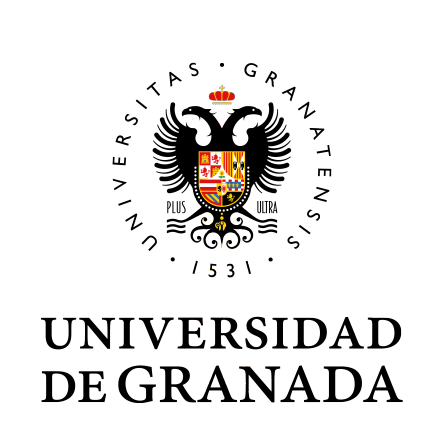
\includegraphics[scale=0.5]{img/ugr.png}\\

        \textsc{\Large \asignatura{}\\[0.2cm]}
        \textsc{MÁSTER CIENCIA DE DATOS E INGENIERÍA DE COMPUTADORES}\\[1cm]

        \noindent\rule[-1ex]{\textwidth}{1pt}\\[1.5ex]
        \textsc{{\Huge \titulo\\[0.5ex]}}
        \textsc{{\Large \subtitulo\\}}
        \noindent\rule[-1ex]{\textwidth}{2pt}\\[2.5ex]

        \end{minipage}

        \vspace{0.3cm}

        \begin{minipage}{\textwidth}

        \centering

        \textbf{Autor}\\ {\autor{} \\ ignaciove@correo.ugr.es}\\[1.5ex]
        \vspace{0.4cm}

        
\includegraphics[scale=0.3]{img/etsiit.jpeg}
        
\includegraphics[scale=0.6]{img/master.png}

        \vspace{0.7cm}
        \textsc{Escuela Técnica Superior de Ingenierías Informática y de Telecomunicación}\\
        \vspace{1cm}
        \textsc{Curso 2020-2021}
    \end{minipage}
\end{titlepage}
% ==============================================================================
    
    \pagenumbering{arabic}    
    \newpage

    % ==============================================================================

    \section{Técnicas de Clasificación}

Como hemos visto en el apartado de EDA, tenemos un conjunto desbalanceado. Por la descripción del problema, cometemos un error mayor cuando clasificamos mal la clase Yes. Por tanto, se podría considerar penalizar más los falsos negativos, de manera que los algoritmos de clasificación intenten cometer menores errores de este tipo. 

\subsection{Algoritmo KNN}

Recordamos los gráficos 1-1 con las clasificaciones, vistos en el EDA.

\begin{figure}[H]\center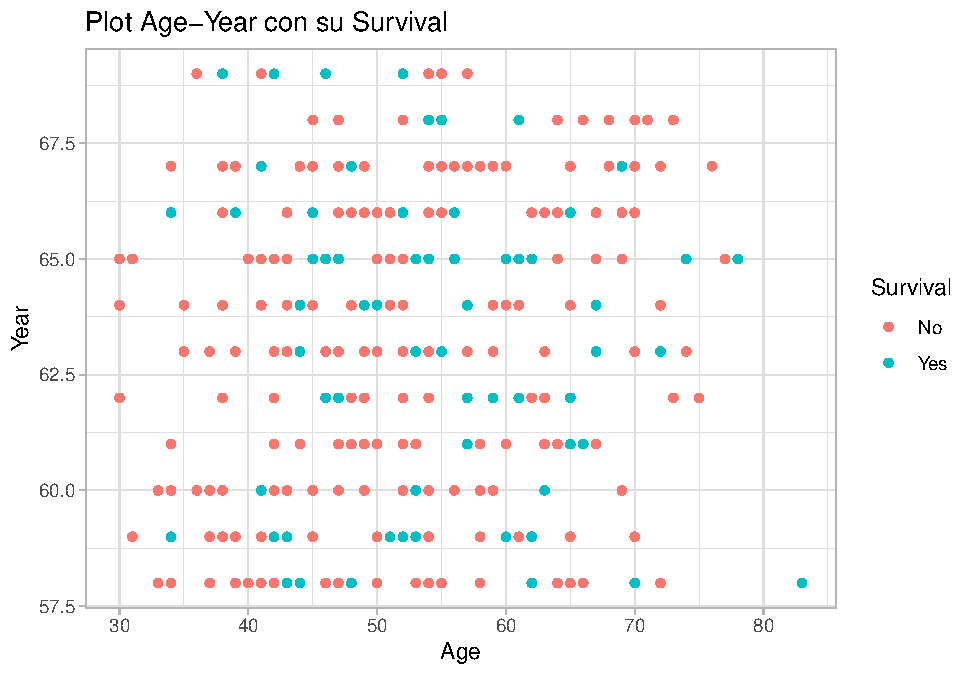
\includegraphics[width=.9\linewidth]{img/Clasificacion_files/figure-latex/unnamed-chunk-5-1}\caption{}\end{figure}

\begin{figure}[H]\center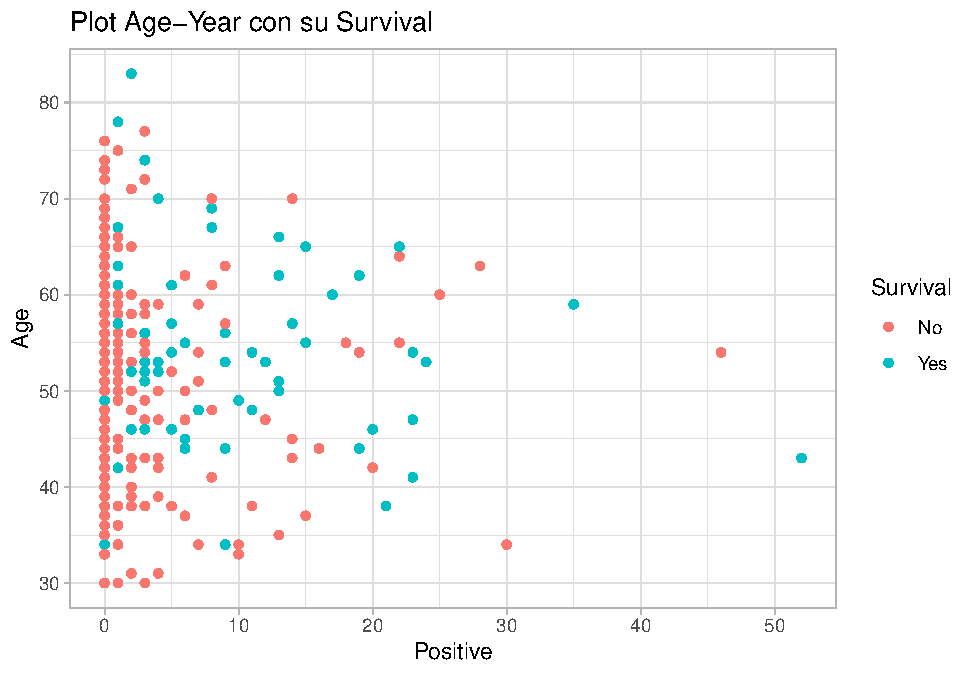
\includegraphics[width=.9\linewidth]{img/Clasificacion_files/figure-latex/unnamed-chunk-5-2}\caption{}\end{figure}

\begin{figure}[H]\center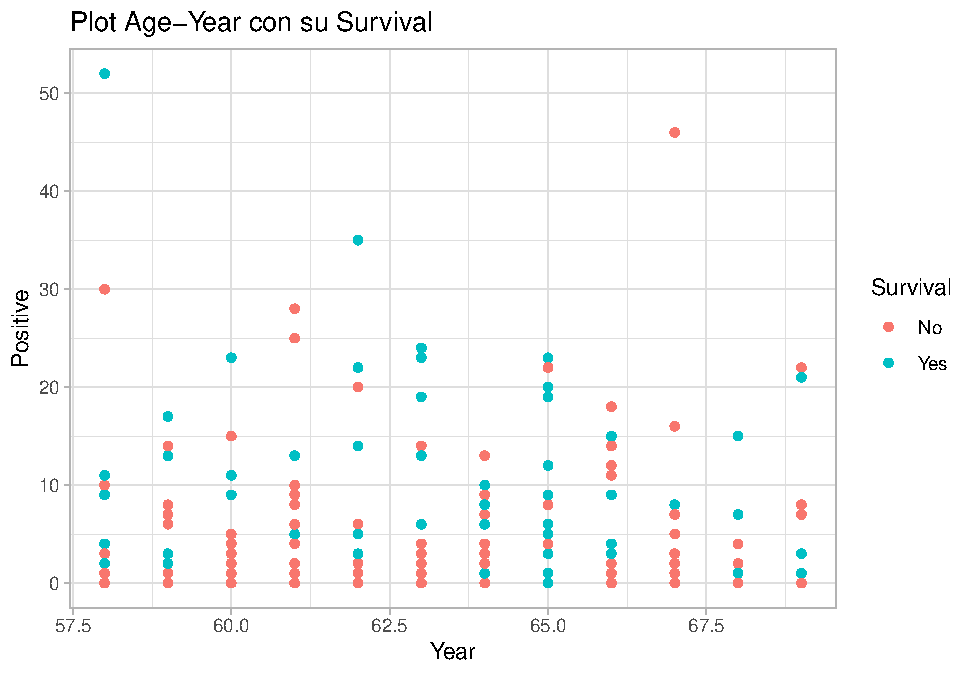
\includegraphics[width=.9\linewidth]{img/Clasificacion_files/figure-latex/unnamed-chunk-5-3}\caption{}\end{figure}

\begin{figure}[H]\center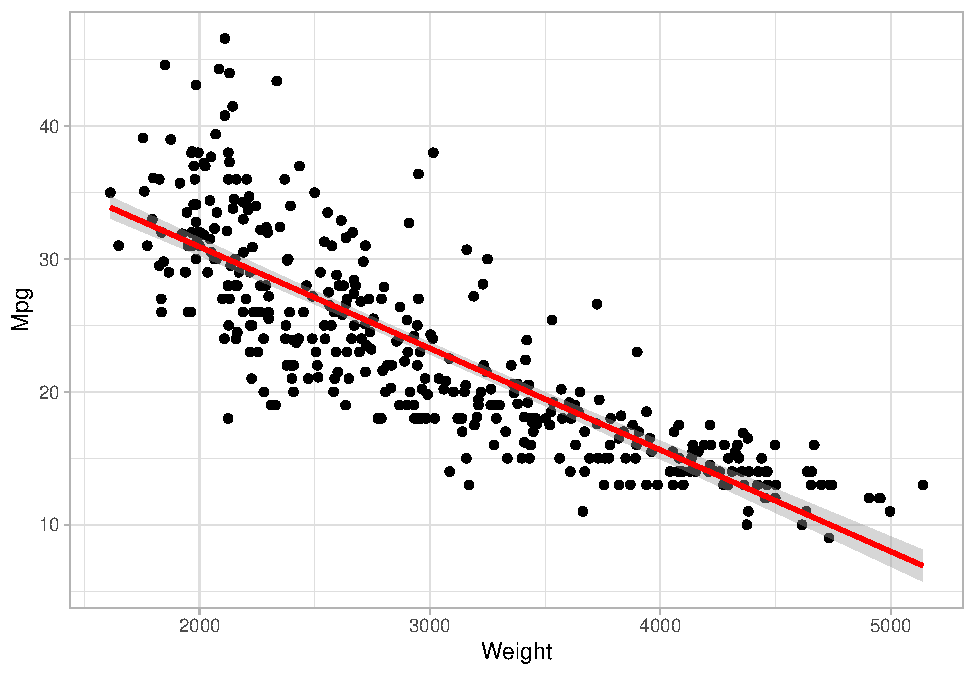
\includegraphics[width=.9\linewidth]{img/Clasificacion_files/figure-latex/unnamed-chunk-6-1}\caption{}\end{figure}

\begin{figure}[H]\center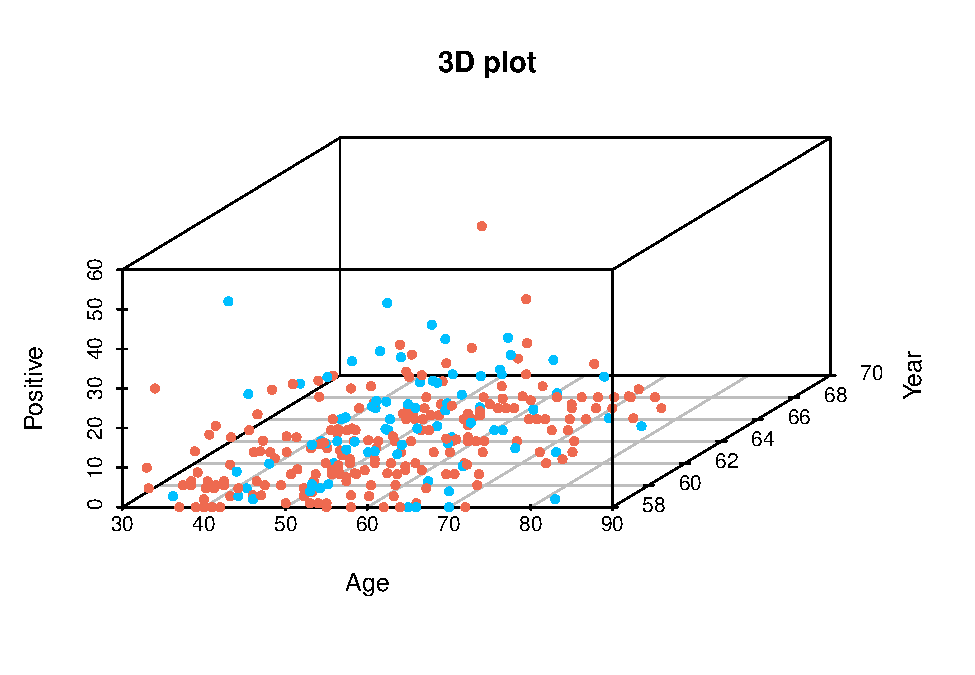
\includegraphics[width=.9\linewidth]{img/Clasificacion_files/figure-latex/unnamed-chunk-6-2}\caption{}\end{figure}

De cara a un algoritmo KNN, apreciamos los datos muy entremezclados, con mayor tendencia a agruparse los no supervivientes que los que sí, pero nada en especial que nos llame la atención.

\vspace{\baselineskip}

Debido a esto vamos a empezar con un valor de K relativamente bajo y vamos a ir aumentándolo poco a poco. Tenemos que tener en cuenta que un K mayor puede ocasionar overfitting, pero usando técnicas de cross-validation podemos minimizar las posibilidades.

Los resultados usando el paquete caret son los siguientes\footnote{Los datos han sido preprocesados con una estandarización antes de aplicar cualquiera de los algoritmos}:
\begin{verbatim}
k-Nearest Neighbors 

275 samples
  3 predictor
  2 classes: 'No', 'Yes' 

No pre-processing
Resampling: Cross-Validated (10 fold) 
Summary of sample sizes: 248, 247, 247, 247, 247, 247, ... 
Resampling results across tuning parameters:

  k   Accuracy   Kappa    
   3  0.6947599  0.2034939
   4  0.6832418  0.1615034
   5  0.6884412  0.1100164
   6  0.6879121  0.1426382
   7  0.6950549  0.0983539
   8  0.7165954  0.1496547
   9  0.7240130  0.1881672
  10  0.7164632  0.1470534
  11  0.7277269  0.1753847
  12  0.7203195  0.1708068
  13  0.7241656  0.1767408
  14  0.7313085  0.2015352
  15  0.7422873  0.2320214

Accuracy was used to select the optimal model using the largest value.
The final value used for the model was k = 15.
\end{verbatim}

Vemos que al estar los datos tan entremezclados ni siquiera con un K pequeño aprende bien, es ya con un K medianamente alto (= 15) donde obtiene mayor accuracy en training.

Una vez más probablemente esto se deba a la gran mezcla de los datos, de forma que necesite la ``opinión'' de un gran número de vecinos para poder predecir con mayor confianza el nuevo valor.

\begin{figure}[H]\center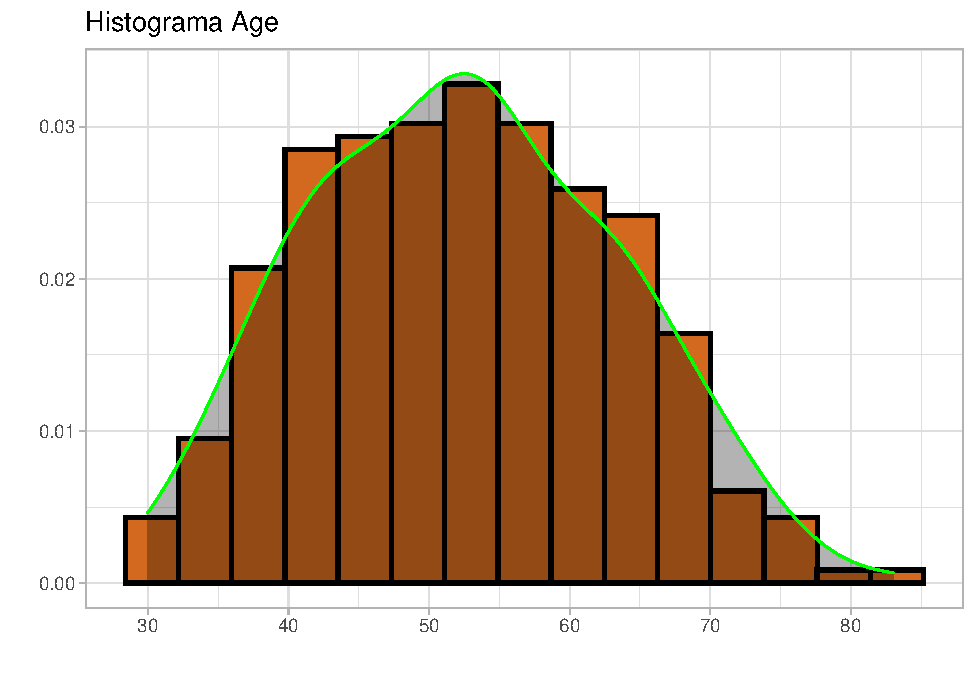
\includegraphics[width=.9\linewidth]{img/Clasificacion_files/figure-latex/unnamed-chunk-10-1}\caption{Predicción con K=15 en training}\end{figure}

Vemos que el uso de un K alto hace que perdamos puntos de Yes. Probablemente al ser minoría el error cometido clasificándolos como No es menor y por eso obtiene mejor accuracy.

\vspace{\baselineskip}

Una evaluación con el subconjunto reservado inicialmente como test nos muestra una calidad extrañamente superior que la de training.

\begin{verbatim}
Test evaluation:
 Accuracy     Kappa 
0.9032258 0.5181347 

Confusion matrix (in test split):
knnPred No Yes
    No  26   2
    Yes  1   2
\end{verbatim}

\begin{figure}[H]\center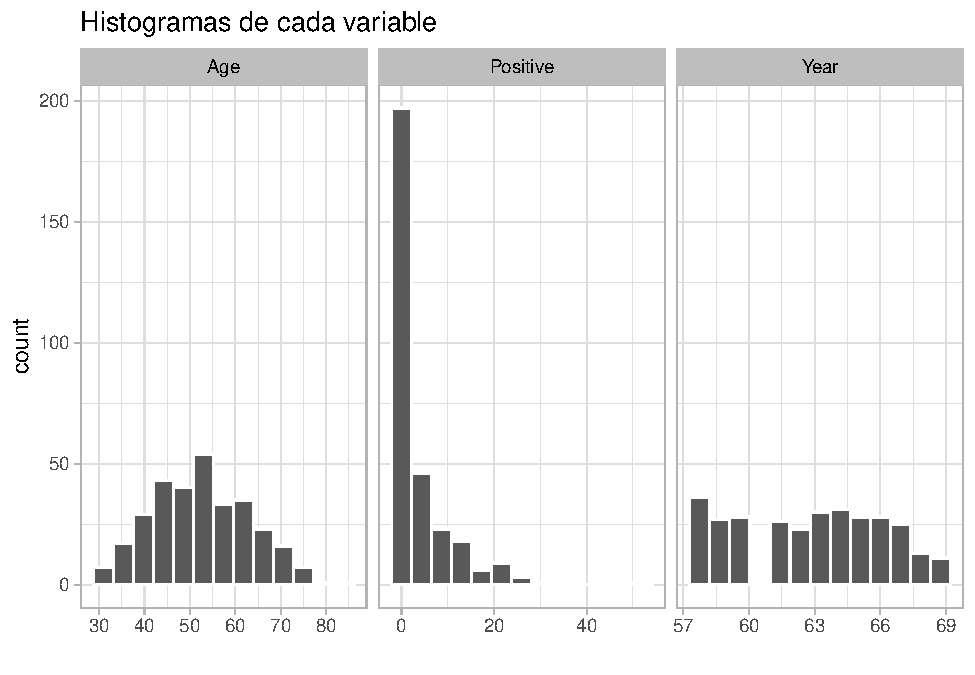
\includegraphics[width=.9\linewidth]{img/Clasificacion_files/figure-latex/unnamed-chunk-9-1}\caption{Matriz de confusión sobre el conjunto de test}\end{figure}

Este comportamiento no es el habitual en aprendizaje automático, parece que casualmente el conjunto de test es bastante fácil de ajustar y por eso se obtienen mejores resultados que en training.
En la sección ?? se muestran las etiquetas. También se vuelve a incidir en la alta presencia de etiquetas \textit{No}.

El valor alto de K hace que se prediga con mayor facilidad este valor de etiqueta y por ese desbalanceo se obtengan tan buenos resultados. En sí es un poco preocupante de cara a la población real de los datos, pero debemos suponer que la muestra que tenemos es representativa y por tanto válida.

Por otro lado, para el problema que nos atañe quizás esto podría ser incluso un hecho positivo, ya que los falsos positivos sería algo que querríamos evitar a toda costa.

\vspace{\baselineskip}

Por comparar, podemos también evaluar con otros valores de K en test. Puesto que hemos obtenido los mejores resultados en training con un K de 15, que es un valor relativamente alto, podemos probar con uno bajo y uno intermedio (3 y 7).

\begin{verbatim}
k-Nearest Neighbors

No pre-processing
Resampling: Cross-Validated (10 fold) 
Summary of sample sizes: 248, 247, 248, 248, 247, 247, ... 
Resampling results:

  Accuracy  Kappa    
  0.697619  0.1988554

Tuning parameter 'k' was held constant at a value of 3
\end{verbatim}

\begin{verbatim}
Test evaluation:
Accuracy     Kappa 
0.8064516 0.1388889

Confusion matrix (in test split):
         test_labels
knn3Pred   No Yes
     No    24   3
     Yes    3   1
\end{verbatim}

\begin{figure}[H]\center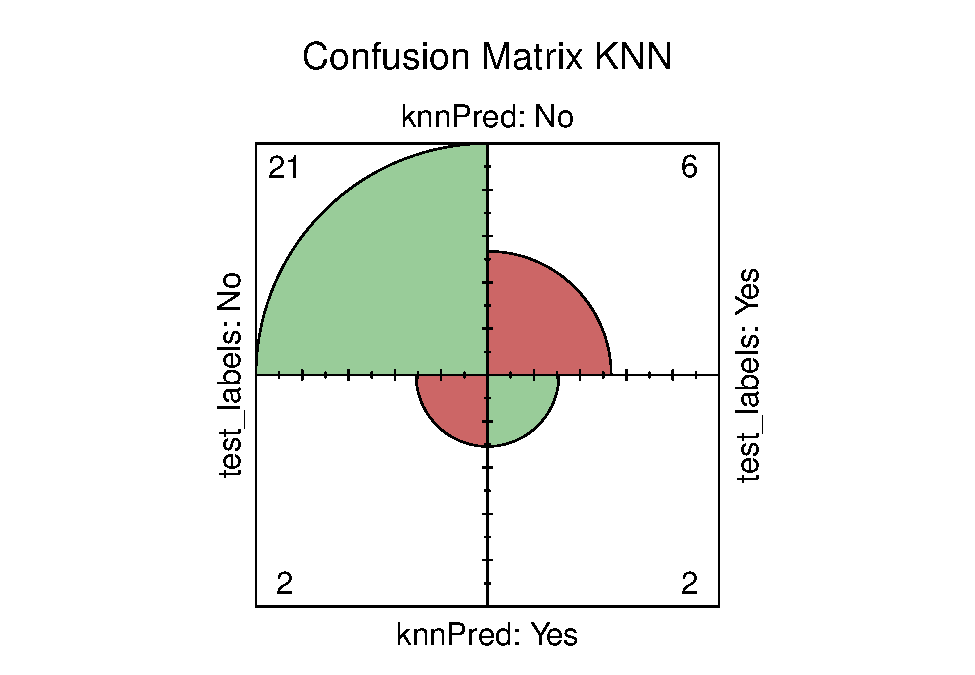
\includegraphics[width=.9\linewidth]{img/Clasificacion_files/figure-latex/unnamed-chunk-12-1}\caption{Matriz de confusión sobre el conjunto de test}\end{figure}

\newpage

\begin{verbatim}
k-Nearest Neighbors 

No pre-processing
Resampling: Cross-Validated (10 fold) 
Summary of sample sizes: 248, 247, 247, 248, 248, 247, ... 
Resampling results:

  Accuracy   Kappa     
  0.6761905  0.08141897

Tuning parameter 'k' was held constant at a value of 7
\end{verbatim}

\begin{verbatim}
Test evaluation:
Accuracy     Kappa 
0.8064516 0.1388889

Confusion matrix (in test split):
        test_labels
knn7Pred No Yes
     No  24   3
     Yes  3   1 
\end{verbatim}

\begin{figure}[H]\center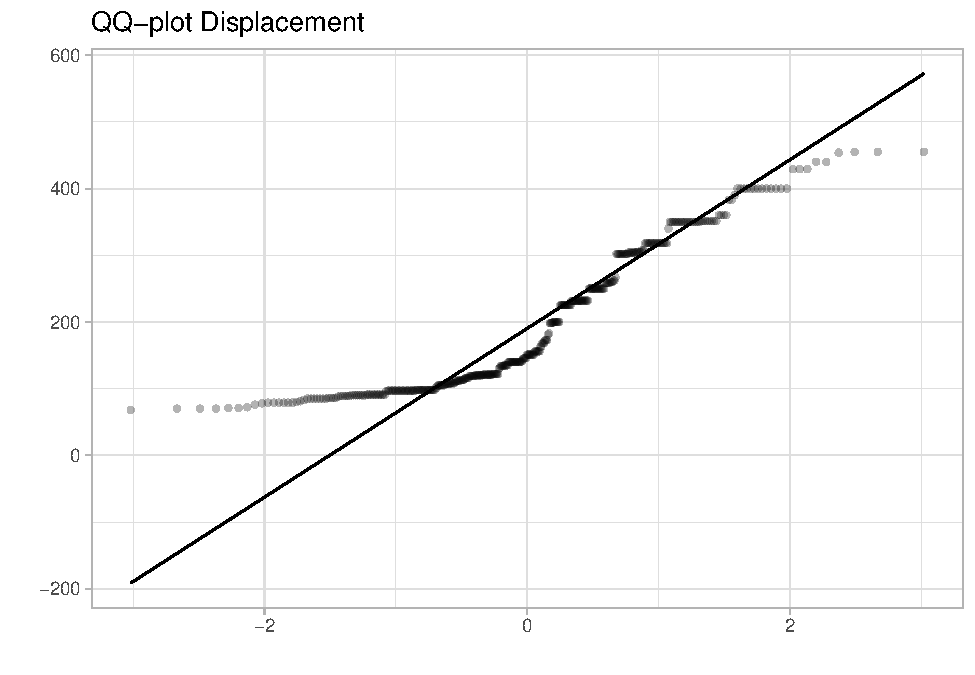
\includegraphics[width=.9\linewidth]{img/Clasificacion_files/figure-latex/unnamed-chunk-14-1}\caption{Matriz de confusión sobre el conjunto de test}\end{figure}

K=7 vemos que es el que más sufre al evaluar en test, y ambos (tal y como nos había indicado la primera ejecución con CV) tienen una calidad bastante inferior (tanto en training como en test) a un K=15.

\subsection{Algoritmo LDA}
\subsubsection{Asunciones}
Comprobamos asunciones:
\begin{enumerate}
    \item \textbf{Distribución aleatoria}: No nos queda más remedio que creer que sí.
    \item \textbf{Cada predictor sigue una distribución normal}: Ya vimos en el EDA que esto no era cierto. El test de Shapiro nos aseguraba que no había normalidad y los QQ-plots nos lo hacían ver claramente. Técnicamente sabiendo esto no deberíamos usar LDA, pero puesto que esto es un proyecto seguimos.
    
    Por otro lado, las variables Age y Year no parecen seguir una distribución demasiado ``rara'' (en comparación con una normal), por lo que es posible que obtengamos resultados de calidad aceptable.
    \item \textbf{Las clases siguen la misma matriz de covarianza}: Lo comprobamos a continuación.
\end{enumerate}

Calculamos la diagonal de la matriz de correlación para cada una de las clases, obteniendo:
\begin{verbatim}
Para clase Yes:
      Age      Year  Positive 
0.9176155 1.0113109 1.6788033 

Para clase No:
      Age      Year  Positive 
1.0756415 0.9752581 0.5448553 
\end{verbatim}

\vspace{\baselineskip}

Estos valores nos parecen indicar que las variables Age y Positive parecen seguir distintas varianzas, pero es preferible asegurarlo con un test estadístico.

Puesto que nuestras variables no siguen una distribución normal, no podemos hacer el test de homogeneidad de Barlett. Utilizamos por tanto el de Levene
\begin{verbatim}
Age:
\end{verbatim}

\begin{tabular}{l|r|r|r}
\hline
  & Df & F value & Pr(>F)\\
\hline
group & 1 & 1.799898 & 0.1807261\\
\hline
 & 304 &  & \\
\hline
\end{tabular}

\begin{verbatim}
Year:
\end{verbatim}

\begin{tabular}{l|r|r|r}
\hline
  & Df & F value & Pr(>F)\\
\hline
group & 1 & 0.0624405 & 0.8028481\\
\hline
 & 304 &  & \\
\hline
\end{tabular}

\begin{verbatim}
Positive:
\end{verbatim}

\begin{tabular}{l|r|r|r}
\hline
  & Df & F value & Pr(>F)\\
\hline
group & 1 & 18.78912 & 1.99e-05\\
\hline
 & 304 &  & \\
\hline
\end{tabular}

Indicándonos que solo se puede asegurar que la variable Positive no tiene homogeneidad entre clases diferentes.

\vspace{\baselineskip}

Gráficamente:

\begin{figure}[H]\center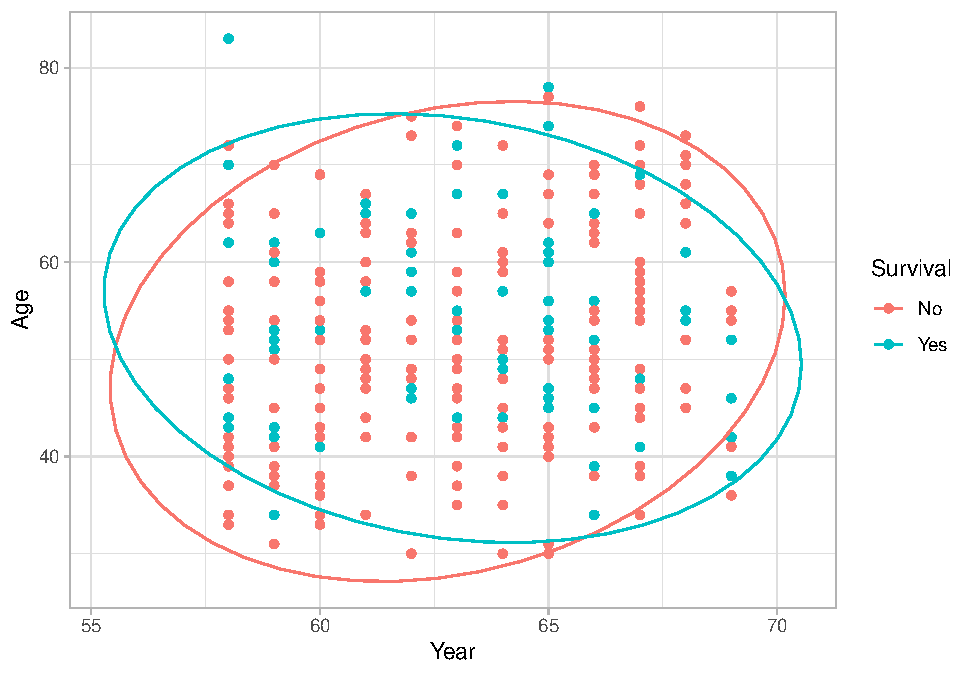
\includegraphics[width=.8\linewidth]{img/Clasificacion_files/figure-latex/unnamed-chunk-17-1}\caption{}\end{figure}

\begin{figure}[H]\center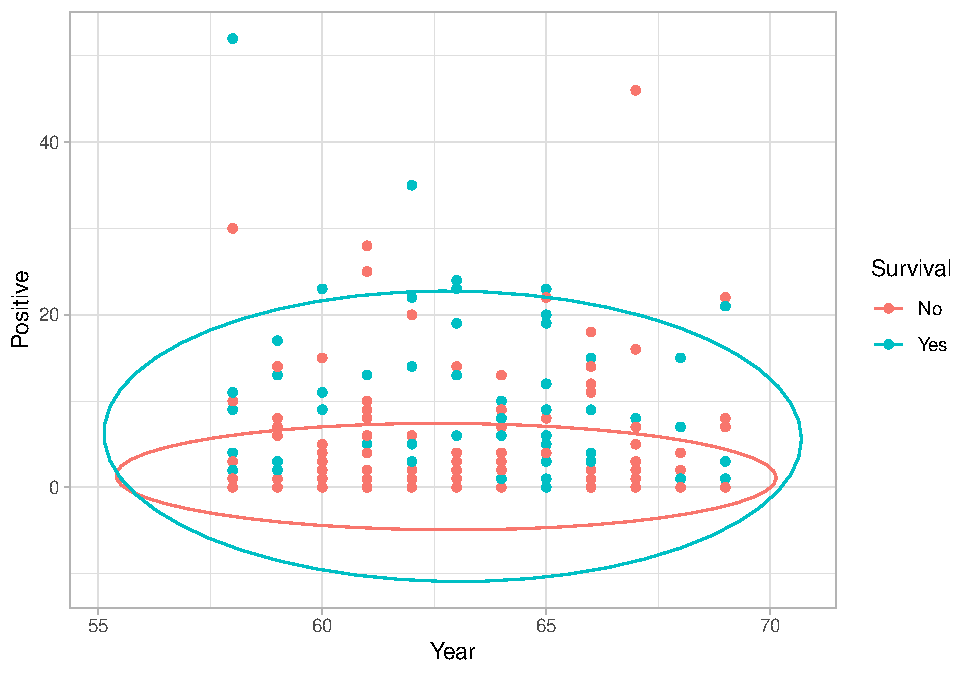
\includegraphics[width=.8\linewidth]{img/Clasificacion_files/figure-latex/unnamed-chunk-17-2}\caption{}\end{figure}

\begin{figure}[H]\center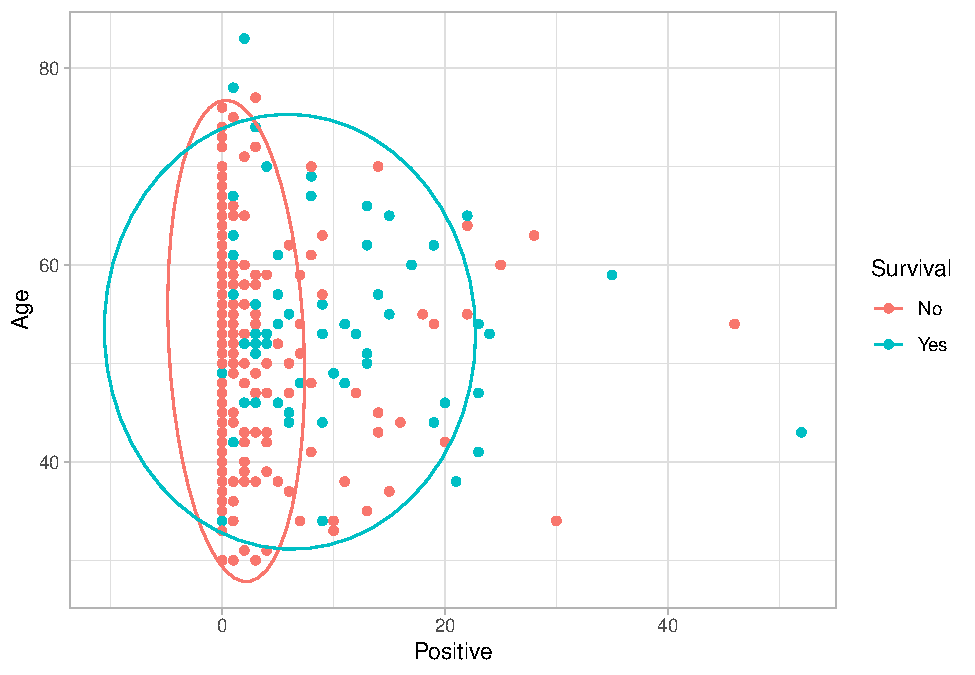
\includegraphics[width=.8\linewidth]{img/Clasificacion_files/figure-latex/unnamed-chunk-17-3}\caption{}\end{figure}

\begin{figure}[H]\center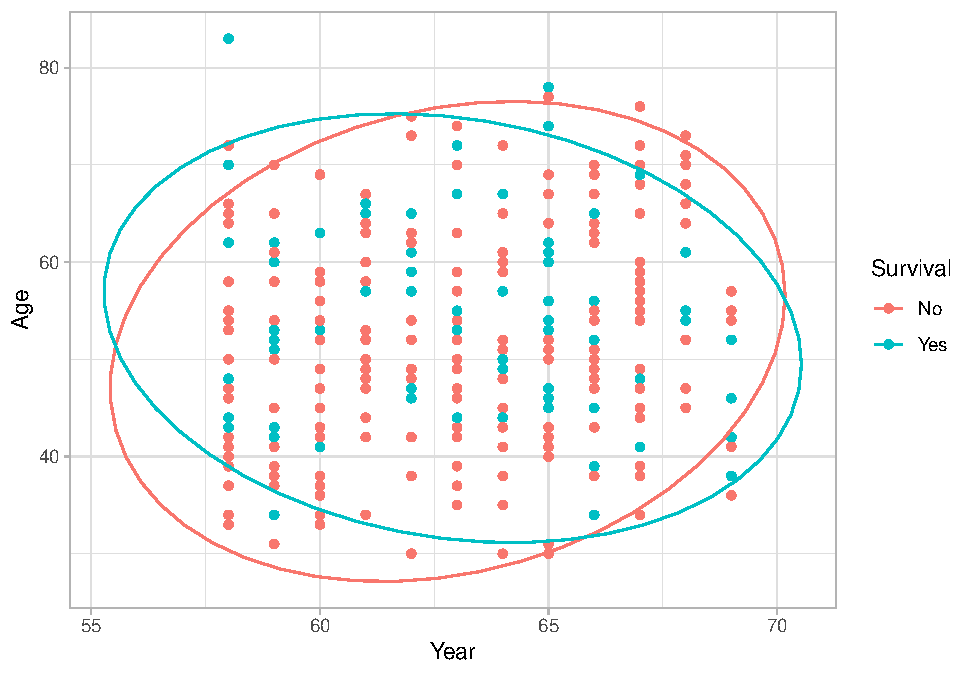
\includegraphics[width=.8\linewidth]{img/Clasificacion_files/figure-latex/unnamed-chunk-18-1}\caption{}\end{figure}

\begin{figure}[H]\center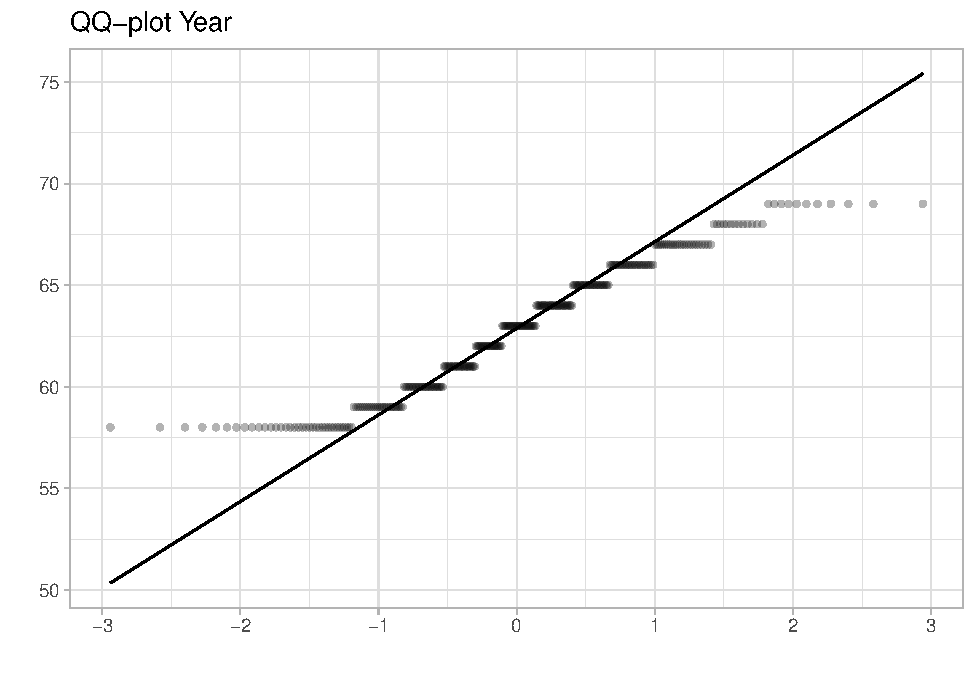
\includegraphics[width=.8\linewidth]{img/Clasificacion_files/figure-latex/unnamed-chunk-18-2}\caption{}\end{figure}

\begin{figure}[H]\center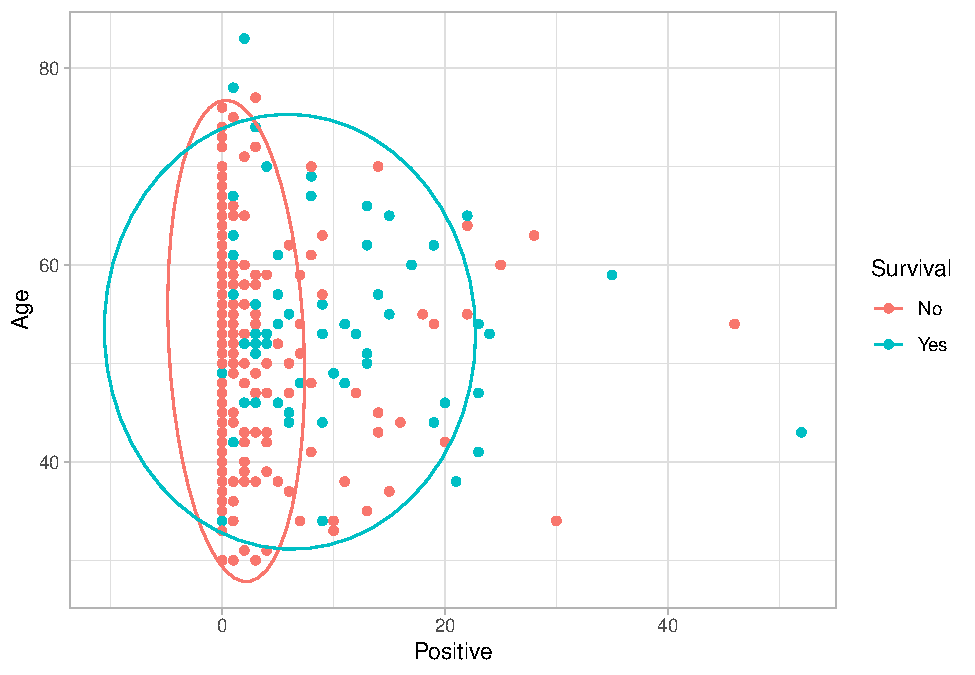
\includegraphics[width=.8\linewidth]{img/Clasificacion_files/figure-latex/unnamed-chunk-18-3}\caption{}\end{figure}

Se nota que la causa de que no se rechace el test para esta variable es la gran cantidad de datos con Positive igual a 0.

\vspace{\baselineskip}

Por tanto para LDA no podemos hacer uso de la variable Positive, puesto que además de la falta de normalidad se incumpliría la asunción número 3, por lo que usamos las otras dos.

\vspace{\baselineskip}

Aunque solo es recomendable, y no son cualidades necesarias para obtener solución en LDA:
\begin{itemize}
    \item Tenemos más instancias que predictores, por varios órdenes de magnitud.
    \item Los predictores son independientes. 
    \item No tenemos varianza cercana a cero.
\end{itemize}

\subsubsection{Aplicación del algoritmo LDA}

\begin{verbatim}
Call:
lda(x, y)

Prior probabilities of groups:
  No  Yes 
0.72 0.28 

Group means:
            Age        Year
No  -0.04141411 0.004845716
Yes  0.11031976 0.021276742

Coefficients of linear discriminants:
            LD1
Age  0.98140853
Year 0.03411981
Cross-Validated (10 fold) Confusion matrix (in test split) 

(entries are percentual average cell counts across resamples)
 
          Reference
Prediction No Yes
       No  72  28
       Yes  0   0
                          
 Accuracy (average) : 0.72
\end{verbatim}

\begin{figure}[H]\center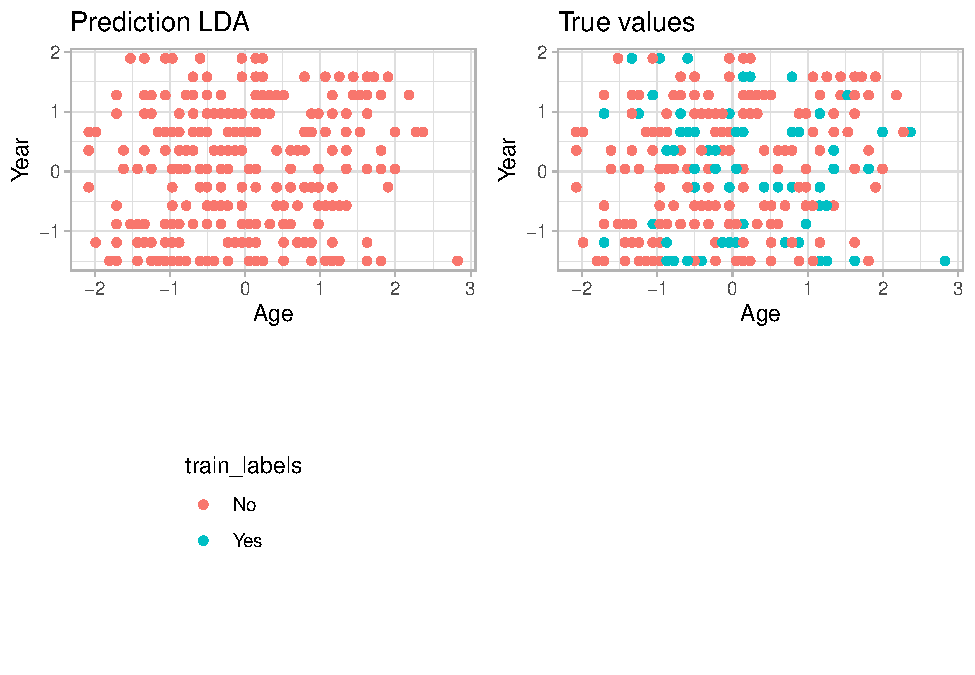
\includegraphics[width=.9\linewidth]{img/Clasificacion_files/figure-latex/unnamed-chunk-22-1}\caption{Predicciones LDA sobre training}\end{figure}

Hacemos un plot del ajuste

\begin{figure}[H]\center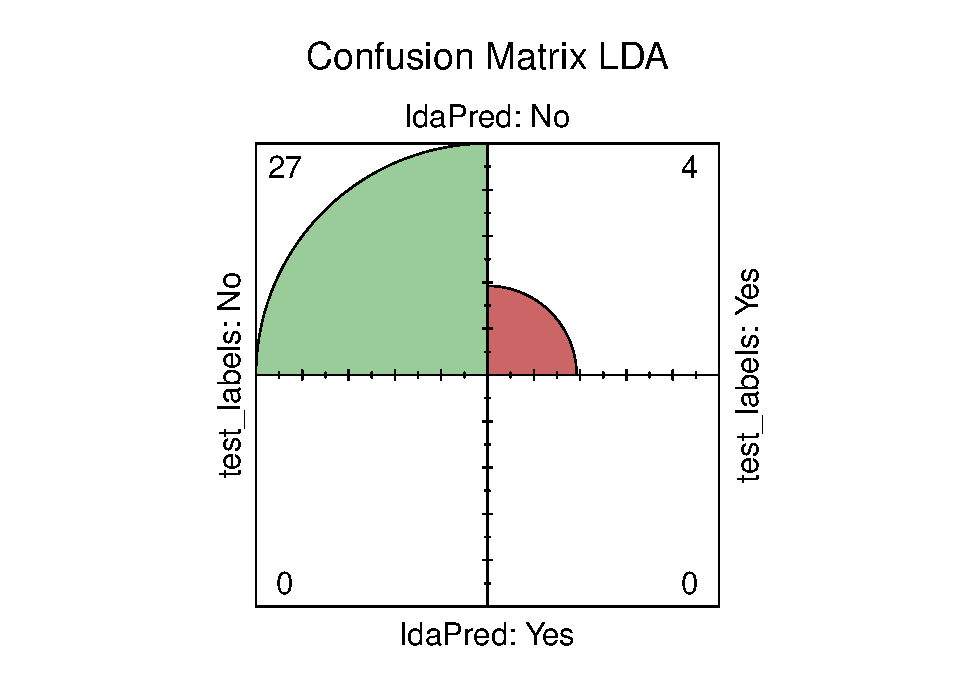
\includegraphics[width=.9\linewidth]{img/Clasificacion_files/figure-latex/unnamed-chunk-23-1}\caption{}\end{figure}

\begin{figure}[H]\center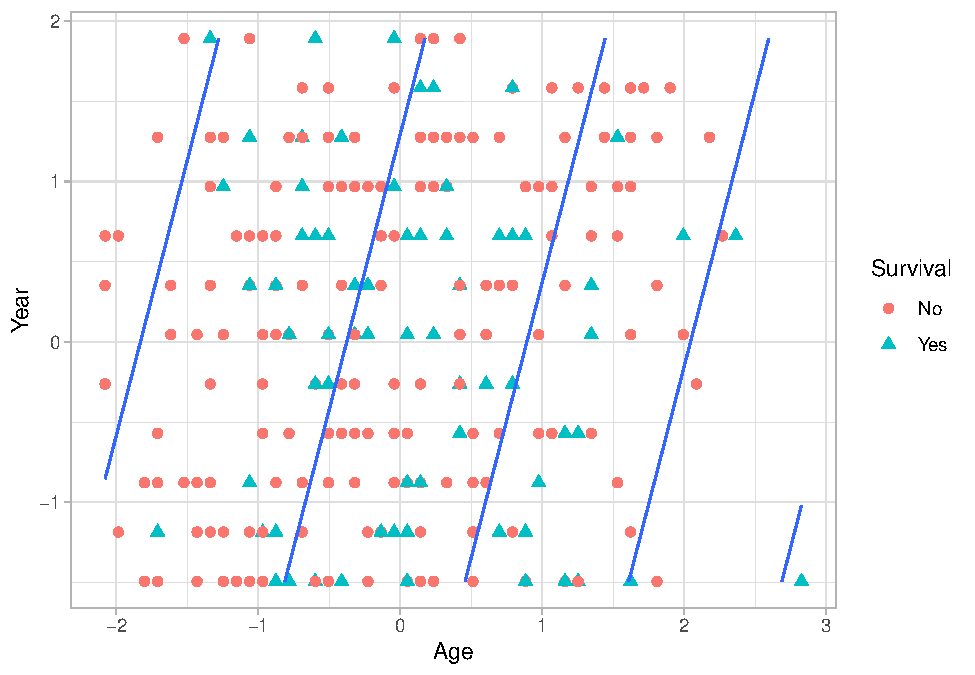
\includegraphics[width=.9\linewidth]{img/Clasificacion_files/figure-latex/unnamed-chunk-24-1}\caption{}\small{Estamos pintando un contorno 3D y por eso nos salen múltiples líneas en el gráfico}\end{figure}

Predecimos en test

\begin{verbatim}
Test evaluation:
Accuracy     Kappa 
0.8709677 0.0000000 

Confusion matrix (in test split):
       test_labels
ldaPred No Yes
    No  27   4
    Yes  0   0
\end{verbatim}

\begin{figure}[H]\center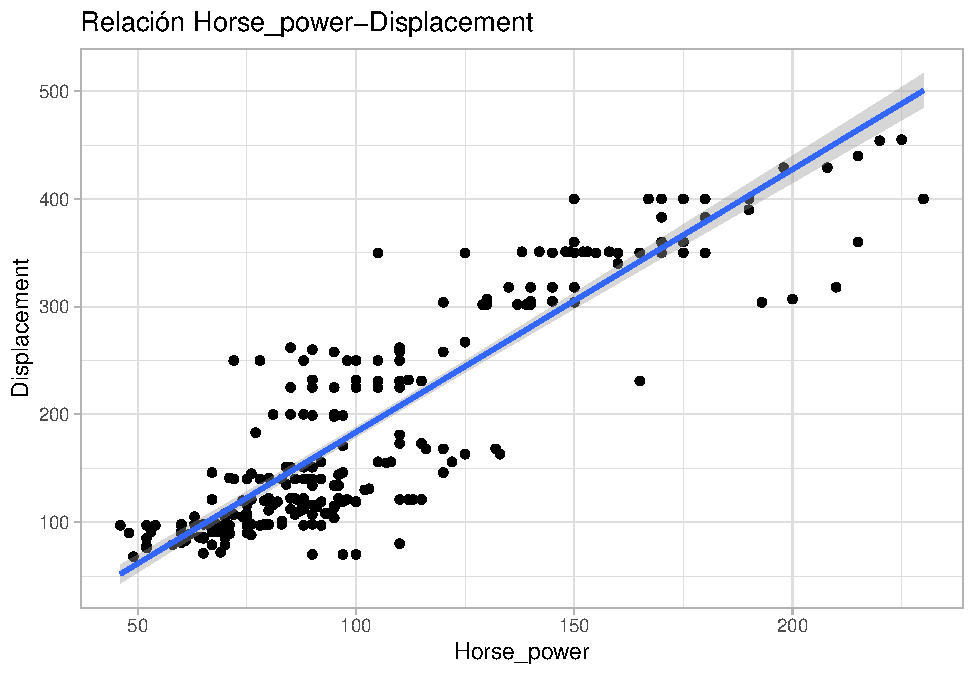
\includegraphics[width=.9\linewidth]{img/Clasificacion_files/figure-latex/unnamed-chunk-21-1}\caption{Matriz de confusión sobre el conjunto de test}\end{figure}

Tenemos un dataset bastante desbalanceado, y LDA no predice para la clase Yes. Con esto se asegura un alto accuracy en nuestro entrenamiento, pero no asegura de que para datos externos vaya a ser así. Pese a ello, no nos queda más remedio que suponer que nuestros datos vienen de la misma muestra aleatoria y por tanto son releventes para la clasificación.

\subsection{Algoritmo QDA}
\subsubsection{Asunciones}

QDA tiene las mismas asunciones de LDA salvo que relaja la norma de que las clases tengan igual covarianza. Esto nos permite usar la variable Positive que habíamos descartado en LDA.

\vspace{\baselineskip}

Por tanto tenemos los requisitos de: 
\begin{enumerate}
    \item Distribución aleatoria.
    \item Distribución normal.
\end{enumerate}

Técnicamente el no cumplir normalidad no imposibilita que se encuentre solución, pero ya no nos lo asegura.

\vspace{\baselineskip}

Adicionalmente tenemos de forma recomendada que: 
\begin{itemize}
    \item El número de predictores debe ser menor que el número de instancias de cada clase. 
    
    Del EDA sabemos que esto es cierto.
    \item Los predictores dentro de cada clase no deben estar correlacionados.
    
    Esto podemos verlo mediante matrices de correlación.
\end{itemize}

\begin{figure}[H]\center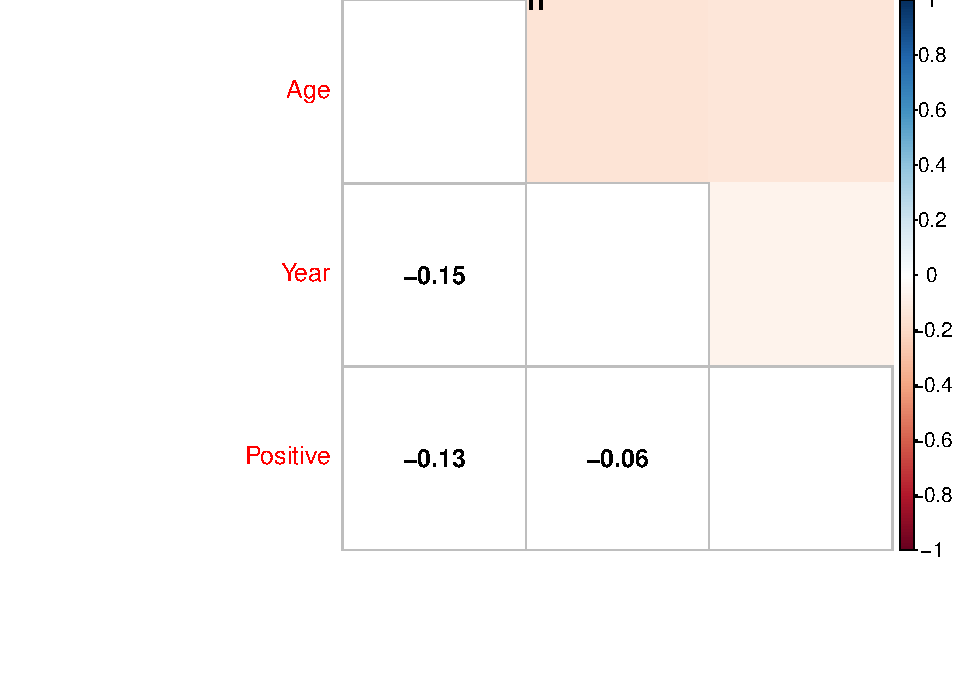
\includegraphics[width=.9\linewidth]{img/Clasificacion_files/figure-latex/unnamed-chunk-25-1}\caption{Matriz de correlación para la clase \textit{Yes}}\end{figure}

\begin{figure}[H]\center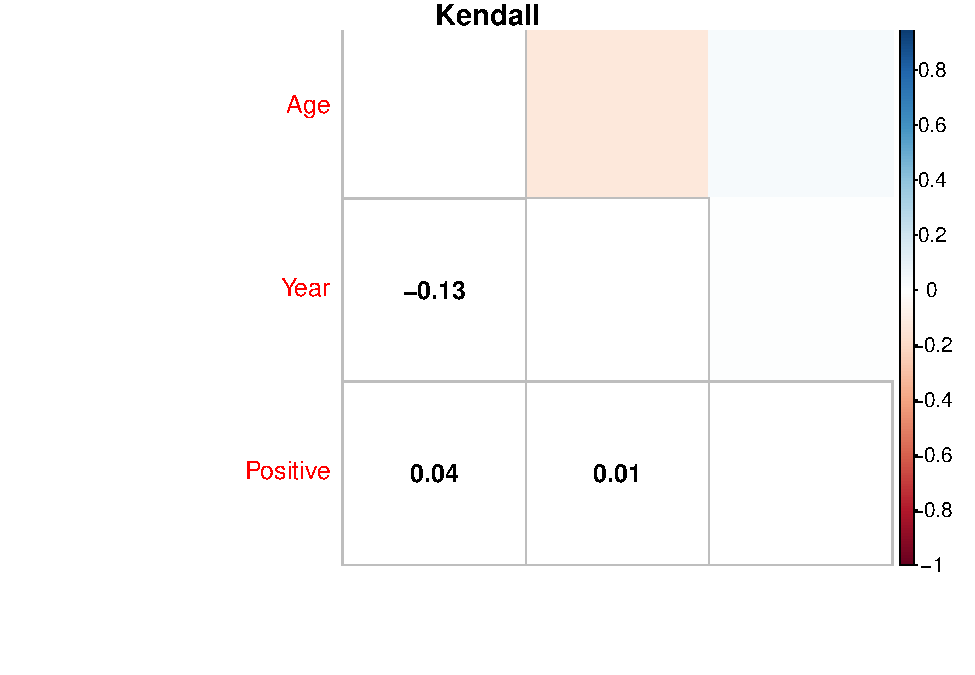
\includegraphics[width=.9\linewidth]{img/Clasificacion_files/figure-latex/unnamed-chunk-25-2}\caption{Matriz de correlación para la clase \textit{Yes}}\end{figure}

\begin{figure}[H]\center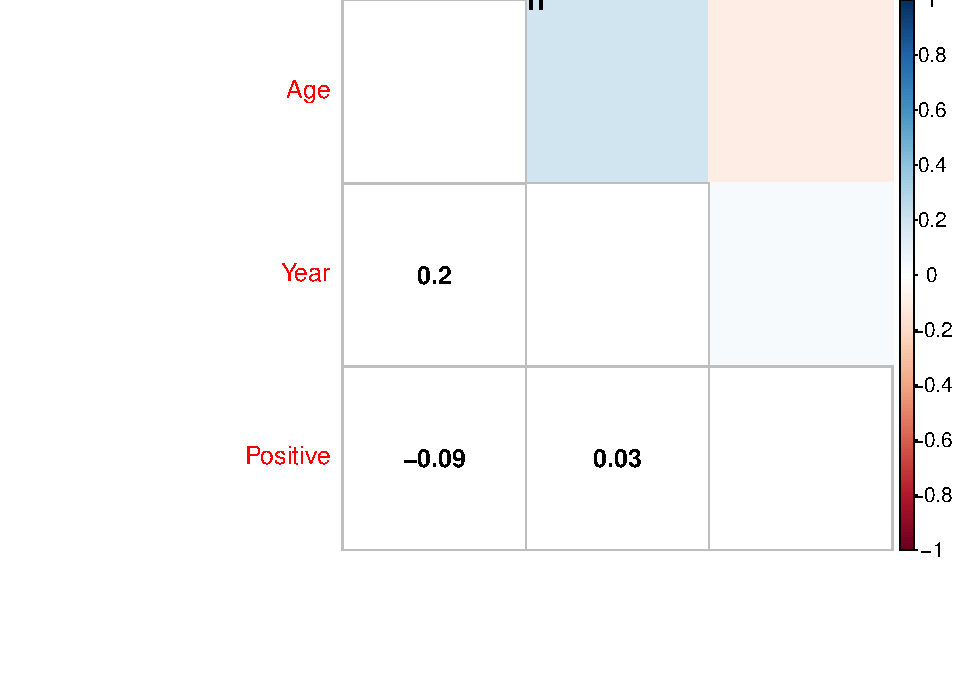
\includegraphics[width=.9\linewidth]{img/Clasificacion_files/figure-latex/unnamed-chunk-26-1}\caption{Matriz de correlación para la clase \textit{No}}\end{figure}

\begin{figure}[H]\center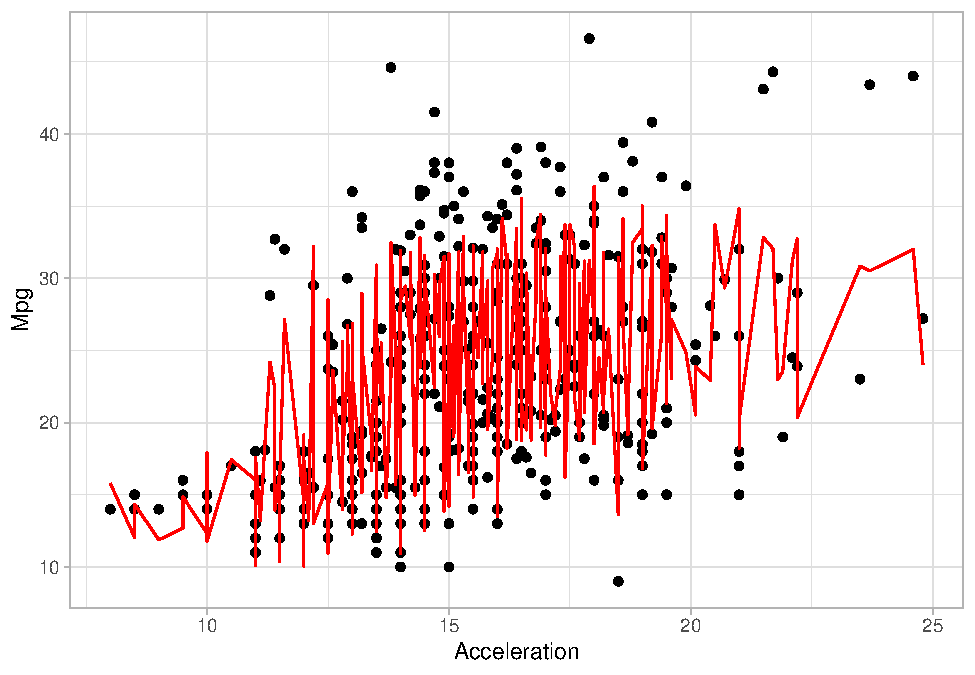
\includegraphics[width=.9\linewidth]{img/Clasificacion_files/figure-latex/unnamed-chunk-26-2}\caption{Matriz de correlación para la clase \textit{Yes}}\end{figure}

\subsubsection{Aplicación del algoritmo QDA}

\begin{verbatim}
Call:
qda(x, y)

Prior probabilities of groups:
  No  Yes 
0.72 0.28 

Group means:
            Age        Year   Positive
No  -0.04141411 0.004845716 -0.1792534
Yes  0.11031976 0.021276742  0.4804648
Cross-Validated (10 fold) Confusion matrix (in test split) 

(entries are percentual average cell counts across resamples)
 
          Reference
Prediction   No  Yes
       No  67.3 21.5
       Yes  4.7  6.5
                            
 Accuracy (average) : 0.7382
\end{verbatim}

\begin{figure}[H]\center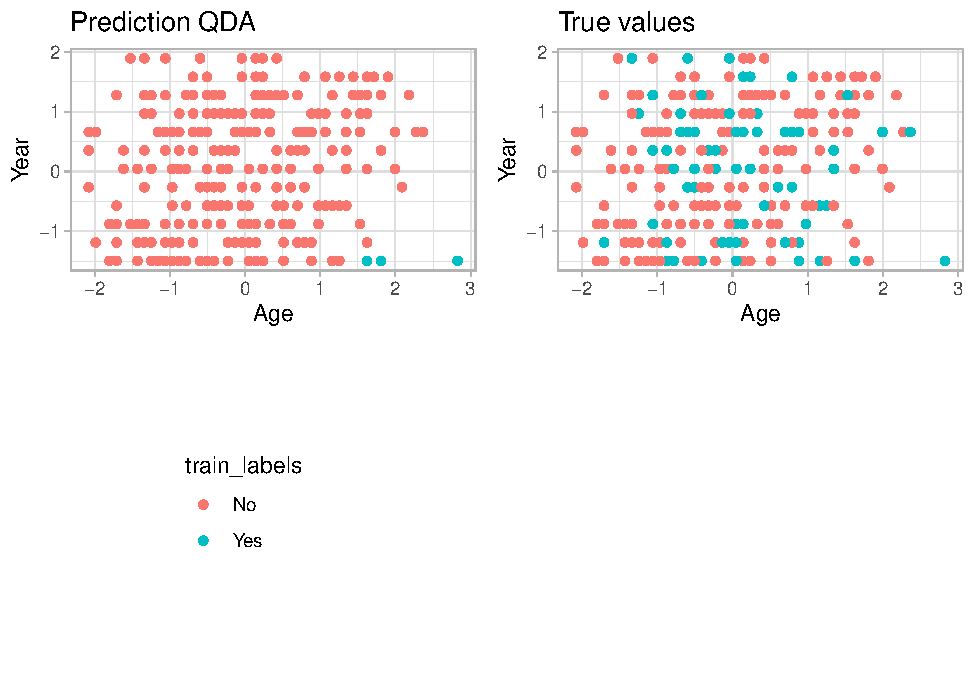
\includegraphics[width=.9\linewidth]{img/Clasificacion_files/figure-latex/unnamed-chunk-30-1}\caption{Predicciones QDA sobre training}\end{figure}


\begin{verbatim}
Test evaluation:
Accuracy     Kappa 
0.8709677 0.2705882

Confusion matrix (in test split):
       test_labels
qdaPred No Yes
    No  26   3
    Yes  1   1
\end{verbatim}

\begin{figure}[H]\center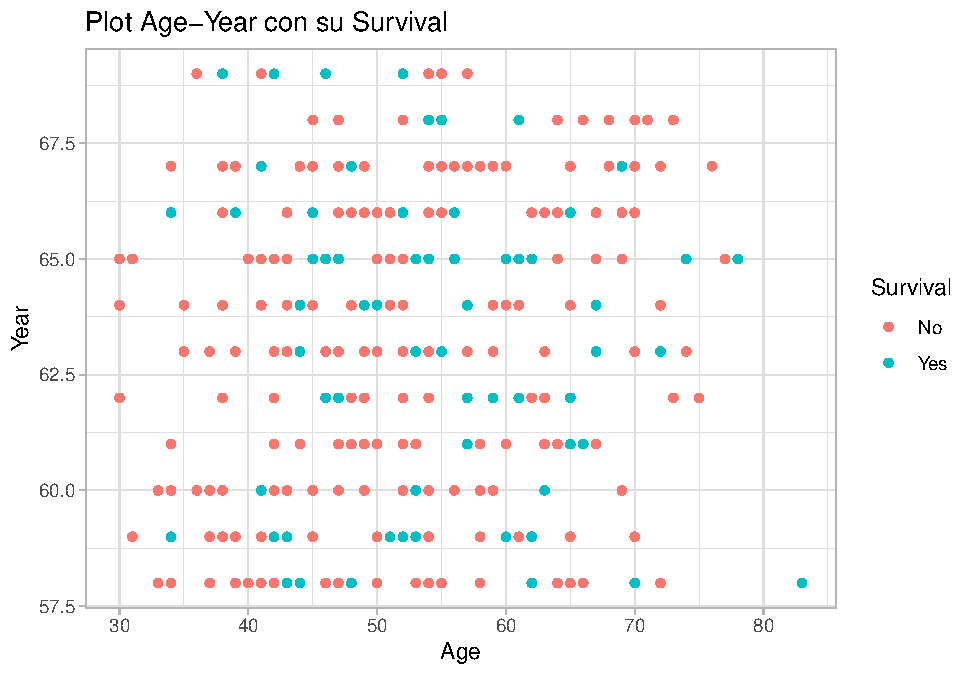
\includegraphics[width=.9\linewidth]{img/Clasificacion_files/figure-latex/unnamed-chunk-29-1}\caption{Matriz de confusión sobre el conjunto de test}\end{figure}

Obtenemos la mismos accuracy que LDA, pero en este caso vemos que sí se predice la clase Yes.

\subsection{Comparativa de algoritmos}
\subsubsection{Para el dataset \textit{haberman}}

Si nos fijamos únicamente en los resultados obtenidos para este problema, los tres algoritmos obtienen el mismo accuracy en nuestro conjunto de test\footnote{Puesto que hemos usado el paquete caret, no podemos comparar con los datos de accuracy que nos proporciona su salida. Los datos aquí mostrados hacen referencia a una evaluación de los modelos devueltos sobre el conjunto inicialmente reservado de test.}. Aunque las etiquetas de este conjunto contienen elementos de ambas clases, podemos ver que se predice mayoritariamente la clase \textit{No}. Como se había mencionado nuestro dataset está bastante desbalanceado, por lo que era más probable que se predijera esa clase con mayor facilidad.

\begin{verbatim}
Etiquetas:
No  No  Yes No  No  No  No  No  Yes No  No  No  No  No  No  No  No  Yes No 
No  No  No  No  No  No  No  No  Yes No  No  No 

Predicciones KNN:
No  No  Yes No  No  No  No  Yes No  No  No  No  No  No  No  No  No  Yes No 
No  No  No  No  No  No  No  No  No  No  No  No 

Predicciones LDA:
No No No No No No No No No No No No No No No No No No No No No No No No No
No No No No No No

Predicciones QDA:
No  No  Yes No  No  No  No  Yes No  No  No  No  No  No  No  No  No  No  No 
No  No  No  No  No  No  No  No  No  No  No  No 
\end{verbatim}

\vspace{\baselineskip}

\begin{verbatim}
Accuracy KNN:
 Accuracy     Kappa 
0.9032258 0.5181347 

Accuracy LDA:
 Accuracy     Kappa 
0.8709677 0.0000000 

Accuracy QDA:
 Accuracy     Kappa 
0.8709677 0.2705882 
\end{verbatim}

\begin{figure}[H]\center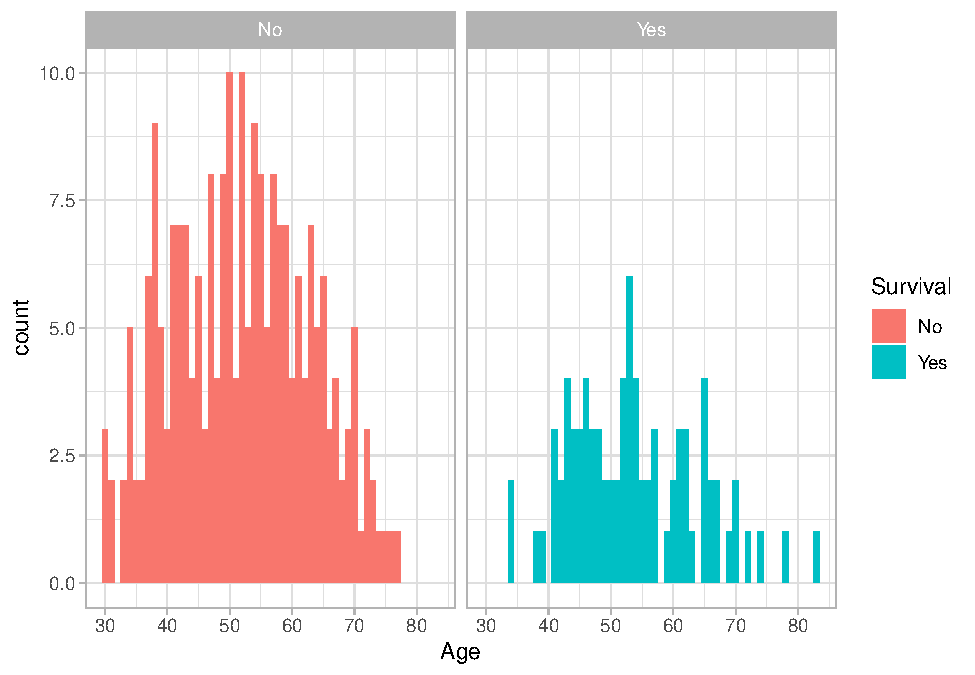
\includegraphics[width=.9\linewidth]{img/Clasificacion_files/figure-latex/unnamed-chunk-33-1}\caption{}\end{figure}

Obtenemos valores de accuracy muy similares, pero diferentes valores de Kappa, siendo en general todos bajos.

\vspace{\baselineskip}

Pese a esto, y ya no solo por tener mejores resultados, sino por no cumplir las asunciones necesarias de obtener resultados de calidad en LDA y QDA, para este problema optaríamos por usar el algoritmo KNN.

A partir de las gráficas 3D de las figuras ?? y ?? se apreció una difícil separación de las clases, por lo que el algoritmo de vecinos más cercanos nos resulta una aproximación más lógica.

\subsubsection{Comparativas generales}

Para comparar la calidad genérica de los algoritmos vamos a aplicar test estadísticos en base a los resultados obtenidos en múltiples datasets.

\vspace{\baselineskip}

Estas son las tablas de resultados que tenemos para test:

\begin{tabular}{l|r|r|r}
\hline
Dataset & out\_test\_knn & out\_test\_lda & out\_test\_qda\\
\hline
appendicitis & 0.8966667 & 0.8690909 & 0.8109091\\
\hline
australian & 0.6838235 & 0.8579710 & 0.8028986\\
\hline
balance & 0.9024546 & 0.8624101 & 0.9167905\\
\hline
bupa & 0.6865775 & 0.6837924 & 0.5991759\\
\hline
contraceptive & 0.5448653 & 0.5091561 & 0.5173102\\
\hline
haberman & 0.7462069 & 0.7481720 & 0.7512903\\
\hline
hayes-roth & 0.5666667 & 0.5500000 & 0.5875000\\
\hline
heart & 0.6692308 & 0.8481481 & 0.8296296\\
\hline
iris & 0.9642857 & 0.9800000 & 0.9733333\\
\hline
led7digit & 0.7510204 & 0.7420000 & 0.6975000\\
\hline
mammographic & 0.7977698 & 0.8241269 & 0.8194042\\
\hline
monk-2 & 0.9743632 & 0.7703433 & 0.9235535\\
\hline
newthyroid & 0.9071429 & 0.9164502 & 0.9629870\\
\hline
pima & 0.7348861 & 0.7709930 & 0.7412403\\
\hline
tae & 0.3838095 & 0.5245833 & 0.5425000\\
\hline
titanic & 0.7850353 & 0.7760304 & 0.7733032\\
\hline
vehicle & 0.6291452 & 0.7813305 & 0.8522409\\
\hline
vowel & 0.6428571 & 0.6030303 & 0.9191919\\
\hline
wine & 0.6959559 & 0.9944444 & 0.9888889\\
\hline
wisconsin & 0.9735023 & 0.9592185 & 0.9519476\\
\hline
\end{tabular}

\vspace{\baselineskip}

Aplicamos el test de Wilcoxon a cada pareja de algoritmos:

\vspace{\baselineskip}

\textbf{LDA vs QDA:} Obtenemos un ranking de 144 para LDA y 96 para QDA, con un p-valor de 0.75 (o nivel de confianza del 25\%).
\begin{verbatim}
V = 96, p-value = 0.7562
alternative hypothesis: true location shift is not equal to 0

  V    V
114 - 96 
\end{verbatim}

Esto nos dice que LDA obtiene mejores resultados pero puesto que el p-value es extremadamente grande no podemos afirmar con garantía estadística que las diferencias entre los tests sean notorias.

\vspace{\baselineskip}

\textbf{LDA vs KNN:} Ahora obtenemos un ranking de 90 para LDA y 120 para QDA, con un p-valor de 0.59 (o nivel de confianza del 41\%).
\begin{verbatim}
V = 120, p-value = 0.5958
alternative hypothesis: true location shift is not equal to 0

 V     V
90 - 120 
\end{verbatim}

Seguimos teniendo un p-valor demasiado grande para poder asegurar la diferencia.

\vspace{\baselineskip}

\textbf{QDA vs KNN:} Por último tenemos un ranking de 69 para LDA y 141 para KNN, con un p-valor de 0.18 (o nivel de confianza del 82\%).
\begin{verbatim}
V = 141, p-value = 0.1893
alternative hypothesis: true location shift is not equal to 0

 V    V
69 - 141
\end{verbatim}

Aunque buscaríamos al menos un 95\% de confianza, podemos afirmar al 82\% que los resultados de ambos algoritmos sí son significativamente diferentes.

\vspace{\baselineskip}
\vspace{\baselineskip}

Una comparativa múltiple de los tres algoritmos con el test de \textbf{Friedman} es la siguiente:

\begin{verbatim}
Friedman rank sum test
Friedman chi-squared = 0.7, 
                  df = 2, 
             p-value = 0.7047
\end{verbatim}

El p-value es mayor que 0.05 por lo que no podemos concluir que haya al menos un par de algoritmos de calidad diferente.

\vspace{\baselineskip}
\vspace{\baselineskip}

Aunque el resultado del test de Friedman ya nos indica que un análisis post-hoc es innecesario, puesto que los resultados que se obtengan no van a asegurar la diferencia en la calidad de los algoritmos, por completitud en la memoria aplicamos el post-hoc de \textbf{Holm}:

\begin{verbatim}
1 = KNN, 2 = LDA, 3 = QDA

Pairwise comparisons using Wilcoxon signed rank exact test 

1    2   
2 1.00 -   
3 0.53 1.00
    
P value adjustment method: holm 
\end{verbatim}

Vemos que los p-value son lo más altos posibles, por lo que carece de sentido intentar diferenciar los algoritmos. Aunque podemos notar, tal y como habíamos visto en los test de Wilcoxon, que la diferencia KNN-QDA probablemente sea mayor que el resto de parejas. \newpage
    \section{Análisis de resultados}

En esta sección se pretenden analizar aquellos resultados más relevantes. Algunos argumentos también se sustentan sobre las tablas completas de experimentos (con información adicional sobre ellos) que se encuentran en la sección \textit{Tablas de resultados}.

% Hay que describir detalladamente todo el proceso algorítmico utilizado, mostrando los resultados de cada uno de los algoritmos utilizados para entrenamiento y test, analizando el comportamiento, y mostrando los flujos/combinaciones de algoritmos de preprocesamiento

\vspace{\baselineskip}

\begin{table}[H]
    \centering
    \begin{tabular}{|l|c|c|c|c|r|}
    \hline
    \textbf{Algoritmo} & \textbf{\shortstack{Selección de \\ características}} & \textbf{\shortstack{Under/Over \\ sampling}} & \multicolumn{1}{l|}{\textbf{\shortstack{Filtrado \\ de ruido}}} & \multicolumn{1}{l|}{\textbf{\shortstack{Selección de \\ instancias}}} & \textbf{\shortstack{TPR \\ x \\ TNR}} \\ \hline
    Decision Tree      & No & RUS  & HME & FCNN  & 0.606 \\ \hline
    Random Forest      & No & RUS  & HME & FCNN  & 0.607 \\ \hline
    PCARD              & -  & RUS  & No  & No    & 0.598 \\ \hline
    kNN-IS             & No & RUS  & HME & No    & 0.526 \\ \hline
    \end{tabular}
    \caption{Flujos de preprocesamiento para los mejores resultados de cada algoritmo tras la optimización de parámetros.}
    \label{final}
\end{table}

Todos los valores de TPR x TNR mostrados son calculados sobre el conjunto de test.

% \subsection{Conclusiones generales}
% Objetivamente la calidad de los resultados es bastante superior a la baseline (cuánto ?), pero no por ello un tanto bajas. La práctica se ha enfocado en evaluar las diferentes combinaciones de técnicas (independientemente del resultado obtenido ?REALLY?). Una posible forma de mejorar sería un ajuste mayor de los hiperparámetros ???

\subsection{Sobre las técnicas de aprendizaje}

En términos de los algoritmos de clasificación, tal y como se muestra en la tabla \ref{final}, obtenemos prácticamente la misma calidad con cualquiera de ellos (con variación de milésimas), siendo ligeramente superior Random Forest (RF) y Árboles de Decisión (DT). Para ambas técnicas el flujo de preprocesamiento coincide, reduciendo enormemente el tamaño del conjunto de datos a un 10\% del tamaño original.

Mediante las tablas \ref{dt} y \ref{rf} vemos que independientemente del preprocesamiento los resultados son muy similares para las dos técnicas, probablemente debido al estar un algoritmo formado como ensamblado del otro. A pesar de esto, vemos que en media RF es más robusto con RUS mientras que DT funciona mejor con ROS.

\vspace{\baselineskip}

Sobre PCARD, aunque la calidad máxima se alcanza con las mínimas técnicas de preprocesamiento (ajustar el desbalanceo es imprescindible en este problema, y los resultados lo demuestran) no llega a ser significativamente inferior que el resto. 

Además, a partir de la tabla \ref{pcard} notamos que las técnicas NCNEdit y FCNN empeoran los resultados frente a no usar ninguna. Creemos que el motivo reside en que al aplicar PCARD PCA antes de entrenar los árboles, se pierde demasiada información al haber reducido el conjunto de datos con los algoritmos de filtrado de ruido y reducción de instancias.
% Qué pasa con HME ??

\vspace{\baselineskip}

Respecto a kNN, notamos peor calidad independientemente de la técnica y parámetros con los que se ha probado. Sin hacer un análisis de la distribución de los datos el razonamiento no está claro, pues al ser un algoritmo basado en distancias si existen alto entremezclado entre los elementos de la clase es de esperar con los pocos valores de k que se ha probado sea insuficiente.

% Es incluso posible que el filtrado de ruido 
% Fijándonos en que obtiene una precisión de 0.887 cuando no se aplica ningún preprocesamiento, deducimos que existen una buena cantidad de puntos entremezclados en el espacio - MEJOR NO PONER

\newpage

\subsection{Sobre las técnicas de selección de características}

Como se dijo anteriormente, hemos aplicado PCA únicamente a los algoritmos donde tiene sentido, pero podemos ver a partir de la tabla \ref{avg} y la de cada algoritmo que los resultados empeoran tras su uso.

\vspace{\baselineskip}

Hacemos notar que PCARD se comporta mejor que los árboles de decisión con PCA, a pesar de acabar teniendo un flujo similar. El razonamiento lo achacamos a la discretización aleatoria (RD) de PCARD, que elige un tamaño de intervalos mejor que el de 32 con el que se han entrenado los árboles.

\vspace{\baselineskip}

A pesar de todo, podríamos considerar si la reducción de dimensionalidad conseguida es aceptable a costa de esa cantidad de empeoramiento. En este problema, pasando de una media de 0,593 a 0,584, que corresponde a una clasificación errónea de $593.000 - 584.000 = 9.000$ instancias más, dada la semántica del problema no parece una pérdida substancial. Si por otro caso tratáramos con un problema médico habría que considerar independientemente el TPR y el TNR antes de aceptar esta conclusión.

\subsection{Sobre las técnicas de balanceo de datos}

No solo RUS ayuda a acelerar la tarea de aprendizaje, también nos da los mejores resultados. Aún así, en media vemos que se comporta peor que ROS, debido probablemente a que su combinación con técnicas de selección de instancias reduce en algunos casos de manera excesiva el conjunto de datos.

\subsection{Sobre las técnicas de reducción de ruido}

Los resultados dan a entender de que el dataset no es de por sí bastante ruidoso, y el posible ruido introducido por las otras técnicas no resulta influyente. No por ello dejamos de apreciar que HME ayuda en la obtención de los mejores valores de TPR x TNR y funciona mejor en este conjunto de datos que NCNEdit.

\subsection{Sobre las técnicas de reducción de instancias}

Vemos que el uso de FCNN apenas altera los resultados, pero no por ello deja de ser útil, pues aplica una reducción en torno al 50\% del conjunto de datos. En una situación de big data como la que nos encontramos esto es totalmente deseable, ya que reducimos tiempo de cómputo y carga en el sistema.

\vspace{\baselineskip}

Finalmente, indicamos que aunque la técnica SSMA sobrepasa el límite de 4GB de memoria impuesto en la práctica, en base a las dos ejecuciones con las que contamos (de los primeros días cuando el límite estaba en 46GB) vemos que la reducción en el número de instancias es extremadamente grande, llegando a obtener subconjuntos de 12.000 y 20.000 instancias.
A pesar de ello en este caso los resultados sí son bastante inferiores respecto a FCNN o no aplicar nada, por lo que concluímos que su uso no es positivo en este conjunto de datos.

\begin{table}
    \centering
    \begin{tabular}{cc|c|c|c|}
    \cline{3-5}
    \multicolumn{1}{l}{\textbf{}} & \textbf{} & \multicolumn{1}{c|}{\textbf{Average}} & \multicolumn{1}{c|}{\textbf{STD}} & \textbf{Max} \\ \hline
    \multicolumn{1}{|c|}{\multirow{3}{*}{Filtrado de ruido}}       & No        & 0.282  & 0.234
    & 0.565    \\ \cline{2-5} 
    \multicolumn{1}{|c|}{}  & HME       & 0.339   & 0.226    & 0.575        \\ \cline{2-5} 
    \multicolumn{1}{|c|}{}  & NCNEdit   & 0.273   & 0.249    & 0.564        \\ \hline
    \multicolumn{1}{|c|}{\multirow{2}{*}{Selección de instancias}} & No        & 0.321  & 0.244    & 0.575        \\ \cline{2-5} 
    \multicolumn{1}{|c|}{}  & FCNN      & 0.277   & 0.219    & 0.574        \\ \hline
    \multicolumn{1}{|c|}{\multirow{2}{*}{Selección de características}} & No        & 0.328  & 0.214    & 0.593        \\ \cline{2-5} 
    \multicolumn{1}{|c|}{}  & PCA      & 0.252    & 0.225    & 0.584        \\ \hline
    \multicolumn{1}{|c|}{\multirow{3}{*}{Balanceo de datos}}       & No        & 0.070  & 0.092    & 0.208        \\ \cline{2-5} 
    \multicolumn{1}{|c|}{}  & ROS       & 0.415   & 0.229    & 0.521        \\ \cline{2-5} 
    \multicolumn{1}{|c|}{}  & RUS       & 0.373   & 0.210    & 0.575        \\ \hline
    \end{tabular}
    \caption{Media de resultados de las diferentes técnicas de preprocesamiento.}
    \label{avg}
\end{table}

\begin{table}
    \centering
    \begin{tabular}{cc|c|c|c|}
    \cline{3-5}
    \multicolumn{1}{l}{\textbf{}} & \textbf{} & \multicolumn{1}{c|}{\textbf{Average}} & \multicolumn{1}{c|}{\textbf{STD}} & \textbf{Max} \\ \hline
    \multicolumn{1}{|c|}{\multirow{3}{*}{Filtrado de ruido}}       & No        & 0.288 & 0.253
    & 0.589    \\ \cline{2-5} 
    \multicolumn{1}{|c|}{}  & HME       & 0.339 &  0.231
    & 0.593        \\ \cline{2-5} 
    \multicolumn{1}{|c|}{}  & NCNEdit   & 0.292 &  0.255
    & 0.584        \\ \hline
    \multicolumn{1}{|c|}{\multirow{2}{*}{Selección de instancias}} & No        & 0.333  & 0.256
    & 0.597        \\ \cline{2-5} 
    \multicolumn{1}{|c|}{}  & FCNN      & 0.289 &  0.231
    & 0.593        \\ \hline
    \multicolumn{1}{|c|}{\multirow{2}{*}{Selección de características}} & No        & 0.341  &  0.241
    & 0.593        \\ \cline{2-5} 
    \multicolumn{1}{|c|}{}  & PCA      & 0.272  & 0.242
    & 0.584        \\ \hline
    \multicolumn{1}{|c|}{\multirow{3}{*}{Balanceo de datos}}       & No        & 0.066  &  0.070
    & 0.215        \\ \cline{2-5} 
    \multicolumn{1}{|c|}{}  & ROS       & 0.426 &  0.136
    & 0.542        \\ \cline{2-5} 
    \multicolumn{1}{|c|}{}  & RUS       & 0.284 &  0.273
    & 0.593        \\ \hline
    \end{tabular}
    \caption{Efectos de las diferentes técnicas de preprocesamiento para árboles de decisión.}
    \label{dt}
\end{table}

\begin{table}
    \centering
    \begin{tabular}{cc|c|c|c|}
    \cline{3-5}
    \multicolumn{1}{l}{\textbf{}} & \textbf{} & \multicolumn{1}{c|}{\textbf{Average}} & \multicolumn{1}{c|}{\textbf{STD}} & \textbf{Max} \\ \hline
    \multicolumn{1}{|c|}{\multirow{3}{*}{Filtrado de ruido}}       & No        & 0.239  & 0.250
    & 0.583    \\ \cline{2-5} 
    \multicolumn{1}{|c|}{}  & HME       & 0.294  & 0.238
    & 0.587        \\ \cline{2-5} 
    \multicolumn{1}{|c|}{}  & NCNEdit   & 0.222  & 0.252
    & 0.585        \\ \hline
    \multicolumn{1}{|c|}{\multirow{2}{*}{Selección de instancias}} & No        & 0.278   & 0.257
    & 0.585        \\ \cline{2-5} 
    \multicolumn{1}{|c|}{}  & FCNN      & 0.224  & 0.229
    & 0.587        \\ \hline
    \multicolumn{1}{|c|}{\multirow{2}{*}{Selección de características}} & No        & 0.316  &  0.258
    & 0.587        \\ \cline{2-5} 
    \multicolumn{1}{|c|}{}  & PCA      & 0.187   & 0.211
    & 0.511        \\ \hline
    \multicolumn{1}{|c|}{\multirow{3}{*}{Balanceo de datos}}       & No        & 0.039  & 0.184
    & 0.196        \\ \cline{2-5} 
    \multicolumn{1}{|c|}{}  & ROS       & 0.353  & 0.273
    & 0.532        \\ \cline{2-5} 
    \multicolumn{1}{|c|}{}  & RUS       & 0.362  & 0.179
    & 0.587        \\ \hline
    \end{tabular}
    \caption{Efectos de las diferentes técnicas de preprocesamiento para Random Forest.}
    \label{rf}
\end{table}

\begin{table}
    \centering
    \begin{tabular}{cc|c|c|c|}
    \cline{3-5}
    \multicolumn{1}{l}{\textbf{}} & \textbf{} & \multicolumn{1}{c|}{\textbf{Average}} & \multicolumn{1}{c|}{\textbf{STD}} & \textbf{Max} \\ \hline
    \multicolumn{1}{|c|}{\multirow{3}{*}{Filtrado de ruido}}       & No        & 0.309   & 0.273
    & 0.597        \\ \cline{2-5} 
    \multicolumn{1}{|c|}{}  & HME       & 0.369   &  0.241
    & 0.595        \\ \cline{2-5} 
    \multicolumn{1}{|c|}{}  & NCNEdit   & 0.286   &  0.290
    & 0.593        \\ \hline
    \multicolumn{1}{|c|}{\multirow{2}{*}{Selección de instancias}} & No        & 0.362   & 0.268
    & 0.597        \\ \cline{2-5} 
    \multicolumn{1}{|c|}{}  & FCNN      & 0.281   & 0.252
    & 0.595        \\ \hline
    \multicolumn{1}{|c|}{\multirow{3}{*}{Balanceo de datos}}       & No        & 0.072   & 0.076
    & 0.186        \\ \cline{2-5} 
    \multicolumn{1}{|c|}{}  & ROS       & 0.496   & 0.325
    & 0.542        \\ \cline{2-5} 
    \multicolumn{1}{|c|}{}  & RUS       & 0.397   & 0.220
    & 0.597        \\ \hline
    \end{tabular}
    \caption{Efectos de las diferentes técnicas de preprocesamiento para PCARD.}
    \label{pcard}
\end{table}

\begin{table}
    \centering
    \begin{tabular}{cc|c|c|c|}
    \cline{3-5}
    \multicolumn{1}{l}{\textbf{}} & \textbf{} & \multicolumn{1}{c|}{\textbf{Average}} & \multicolumn{1}{c|}{\textbf{STD}} & \textbf{Max} \\ \hline
    \multicolumn{1}{|c|}{\multirow{3}{*}{Filtrado de ruido}}       & No        & 0.292  & 0.159
    & 0.491    \\ \cline{2-5} 
    \multicolumn{1}{|c|}{}  & HME       & 0.354   & 0.193
    & 0.525        \\ \cline{2-5} 
    \multicolumn{1}{|c|}{}  & NCNEdit   & 0.294  & 0.200
    & 0.492        \\ \hline
    \multicolumn{1}{|c|}{\multirow{2}{*}{Selección de instancias}} & No        & 0.313    &  0.195
    & 0.525        \\ \cline{2-5} 
    \multicolumn{1}{|c|}{}  & FCNN      & 0.313   &  0.165
    & 0.521        \\ \hline
    \multicolumn{1}{|c|}{\multirow{2}{*}{Selección de características}} & No        & 0.328    & 0.177
    & 0.525        \\ \cline{2-5} 
    \multicolumn{1}{|c|}{}  & PCA      & 0.299   & 0.188
    & 0.516        \\ \hline
    \multicolumn{1}{|c|}{\multirow{3}{*}{Balanceo de datos}}       & No        & 0.103     &  0.038
    & 0.235        \\ \cline{2-5} 
    \multicolumn{1}{|c|}{}  & ROS       & 0.386  & 0.180
    & 0.432        \\ \cline{2-5} 
    \multicolumn{1}{|c|}{}  & RUS       & 0.448  & 0.167
    & 0.525        \\ \hline
    \end{tabular}
    \caption{Efectos de las diferentes técnicas de preprocesamiento para kNN.}
    \label{knn}
\end{table} \newpage
    \section{Conclusiones}

\begin{table}[H]
    \centering
    \begin{tabular}{|l|c|c||c|c|c|}
        \hline
        \textbf{Método}  & \textbf{Accuracy} & \textbf{Kappa} & \multicolumn{1}{l|}{\textbf{Specificity}} & \multicolumn{1}{l|}{\textbf{Sensitivity}} & \multicolumn{1}{l|}{\textbf{F-measure}} \\ \hline
        MPQA             & 64.5              & 0.299          & 0.591                                   & 0.768                                & 0.566                                   \\ \hline
        SentiWordNet     & 55.8              & 0.117          & 0.657                                   & 0.525                                & 0.664                                   \\ \hline
        SenticNet        & 58.3              & 0.167          & 0.559                                   & 0.637                                & 0.481                                   \\ \hline \hline

        MPQA             & 70.5              & 0.415          & 0.649                                   & 0.800                                & 0.666                                   \\ \hline
        SentiWordNet     & 52.5              & 0.05          & 0.572                                   & 0.515                                & 0.642                                   \\ \hline
        SenticNet        & 57.1              & 0.143          & 0.577                                   & 0.566                                & 0.587                                   \\ \hline \hline

        Redes Neuronales & 82.5              & 0.65           & 0.854                                   & 0.800                                & 0.832                                   \\ \hline
        Random Forest    & 91.0              & 0.82           & 0.870                                   & 0.950                                & 0.913                                   \\ \hline
        \end{tabular}
    \caption{Tabla de resultados generales.}
\end{table}

Los resultados nos muestran una clara victoria de las técnicas de clasificación frente a los diccionarios.

Ambas heurísticas utilizadas en los diccionarios muestran efectos pobres, donde se ve una predicción excesiva de un solo sentimiento (dependiente según el lexicon). Con la segunda vemos que la predicción está más balanceada, mayormente para SenticNet, pero por desgracia esto no hace que mejore su accuracy, aunque sí el F-score.
A pesar de esto la mejoría si es notoria en el corpus MPQA.

\vspace{\baselineskip}

Los valores de \textit{specificity} y \textit{sensitivity} nos muestran las tasas de verdaderos negativos/positivos respectivamente. A partir de ellas vemos una mayor tendencia general de los diferentes métodos a valorar positivamente cada una de las reviews.

    % ==============================================================================

    \setlength{\parskip}{1em}
    \newpage
\end{document}

% ==============================================================================
% ==============================================================================